\documentclass[letterpaper, 10pt]{article}

\usepackage[noadjust]{cite}
\usepackage{color}
\usepackage{amsmath}
\usepackage{graphicx}
\usepackage{caption}
\usepackage{subcaption}
\usepackage{cuted}
% \usepackage{hyperref}
\usepackage[nameinlink]{cleveref}
\usepackage[flushleft, para]{threeparttable}
\usepackage{multirow}
\usepackage{booktabs}
\usepackage{nth}
\usepackage{afterpage}
\usepackage{contour}

\usepackage{pgf}
\usepackage{tikz}
\usepackage{circuitikz}
\usepackage{pgfplots}
\pgfplotsset{compat = 1.12}

\usetikzlibrary{datavisualization.formats.functions}
\usetikzlibrary{plotmarks}
\usetikzlibrary{math}
\usetikzlibrary{calc}
\usetikzlibrary{spy}
\usetikzlibrary{positioning}
\usetikzlibrary{intersections}
\usetikzlibrary{decorations.text}
\usetikzlibrary{external}
\usetikzlibrary{patterns}
\usetikzlibrary{arrows.meta}
\usetikzlibrary{arrows}
\usetikzlibrary{matrix}

\tikzexternalize

\pgfplotsset{
    legend image with text/.style={
        legend image code/.code={%
            \node[anchor=center] at (0.3cm,0cm) {#1};
        }
    },
}

\mathchardef\myhyphen="2D

\begin{document}

\ifpdf
\DeclareGraphicsExtensions{.pdf, .jpg, .tif}
\else
\DeclareGraphicsExtensions{.eps, .jpg}
\fi

\tikzsetexternalprefix{images/tikz/}

\begin{figure}
  \centering
  \tikzsetnextfilename{tikz-IM-drawing}
  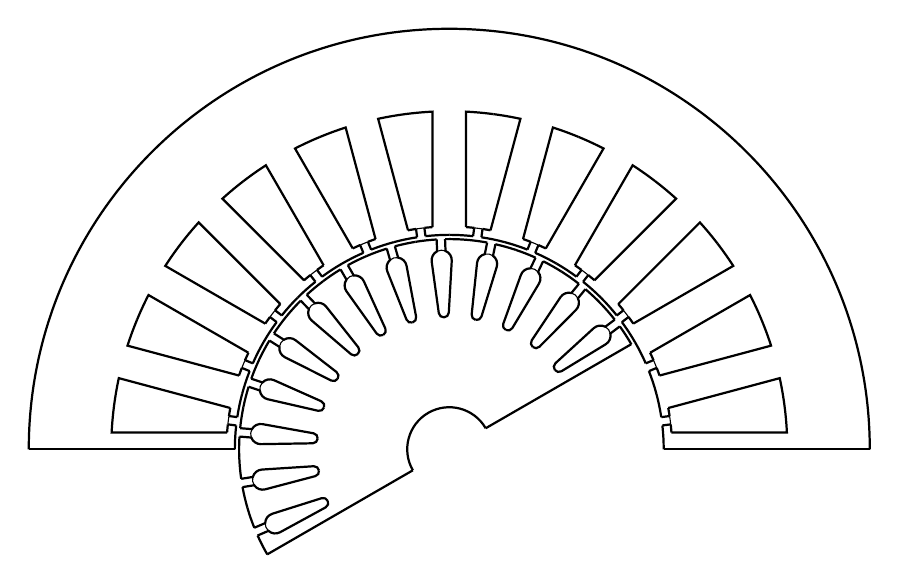
\begin{tikzpicture} [scale = 0.1]
  	\def\ris{27.23}			% stator inner radius
	\def\ros{53.4}			% stator outer radius
	\def\rir{5.34}			% rotor inner radius
	\def\ror{26.695}		% rotor outer radius
	\def\P{2}				% number of pole pairs, draw only one pole pair
	\def\thetar{30}		% rotor position
	
	\def\Qs{24}				% total number of stator slots
	\def\Qr{26}				% total number of rotor slots
	\pgfmathsetmacro{\qs}{\Qs / \P}
	\pgfmathsetmacro{\qr}{\Qr / \P}
	
	\def\sws{1.068}			% stator slot width
	\def\swr{1.07}			% rotor slot width
	
	\def\dtangs{1.068}		% stator teeth tang depth
	\def\cws{10.47}			% stator core back width
	\def\tws{4.271}			% stator teeth width
	
	\def\dbarco{2.67}		% bar outer center depth
	\def\dbarcc{6.62}		% distance between bar edge centers, from c1 to c2
	\def\rco{1.28}			% bar outer radius
	\def\rci{0.64}			% bar inner radius
	
	\def\thetaStatorSlot{asin(0.5 * \sws / \ris) * 2.0}		% stator slot angle
	\def\thetaRotorSlot{asin(0.5 * \swr / \ror) * 2.0}		% rotor slot angle
	
	\def\thetaStatorSlotTang{asin(0.5 * \sws / (\ris + \dtangs)) * 2.0}			% stator slot angle at the tang depth
	\def\thetaStatorSlotTangEnd{asin(0.5 * \tws / (\ris + \dtangs)) * 2.0}		% stator slot end angle at the tang depth
	\def\thetaStatorSlotBottomEnd{asin(0.5 * \tws / (\ros - \cws)) * 2.0}		% stator slot end angle at the slot bottom
	
	\def\thetaRotorSlotTang{asin(0.5 * \swr / \rco) * 2.0}						% rotor slot angle at the tang depth, referring to bar outer center, not machine center
	\def\thetaRotorSlotTangXtoCo{sqrt(\rco * \rco - 0.25 * \swr * \swr)}			% x coordinate of the tang, referring to bar outer center
	\def\thetaRotorSlotWedge{asin((\rco - \rci) / \dbarcc) * 2.0}
	\def\thetaRotorSlotBottomXtoCi{\rci * cos(90 + 0.5 * \thetaRotorSlotWedge)}
	\def\thetaRotorSlotBottomYtoCi{\rci * sin(90 + 0.5 * \thetaRotorSlotWedge)}
	
	% if P == 1, comment the following four lines
	\draw [thick] (       0 : \ris) -- (       0 : \ros);
	\draw [thick] (360 / \P : \ris) -- (360 / \P : \ros);
	\draw [thick] (           \thetar : \rir) -- (           \thetar : \ror);
	\draw [thick] (360 / \P + \thetar : \rir) -- (360 / \P + \thetar : \ror);
	
    \draw [thick] (\ros, 0) arc [start angle = 0, end angle = 360 / \P, radius = \ros];
    \draw [thick] (\thetar : \rir) arc [start angle = \thetar, end angle = {\thetar + 360 / \P}, radius = \rir];
    
    \foreach \s in {1, 2, ..., \qs} {
    	% draw teeth surface
    	\draw [thick] ({360 * (\s - 1) / \Qs} : \ris) arc [start angle = {360 * (\s - 1) / \Qs}, end angle = {180 * (2 * \s - 1) / \Qs - 0.5 * \thetaStatorSlot}, radius = \ris];
		\draw [thick] ({360 * \s / \Qs} : \ris) arc [start angle = {360 * \s / \Qs}, end angle = {180 * (2 * \s - 1) / \Qs + 0.5 * \thetaStatorSlot}, radius = \ris];
		
		% draw slot openning
		\draw [thick] ({180 * (2 * \s - 1) / \Qs - 0.5 * \thetaStatorSlot} : \ris) -- ({180 * (2 * \s - 1) / \Qs - 0.5 * \thetaStatorSlotTang} : {\ris + \dtangs});
		\draw [thick] ({180 * (2 * \s - 1) / \Qs + 0.5 * \thetaStatorSlot} : \ris) -- ({180 * (2 * \s - 1) / \Qs + 0.5 * \thetaStatorSlotTang} : {\ris + \dtangs});
		
		% draw winding area
		\draw [thick] ({180 * (2 * \s - 1) / \Qs - 0.5 * \thetaStatorSlotTang} : {\ris + \dtangs}) arc [start angle = {180 * (2 * \s - 1) / \Qs - 0.5 * \thetaStatorSlotTang}, end angle = {360 * (\s - 1) / \Qs + 0.5 * \thetaStatorSlotTangEnd}, radius = {\ris + \dtangs}];
		\draw [thick] ({180 * (2 * \s - 1) / \Qs + 0.5 * \thetaStatorSlotTang} : {\ris + \dtangs}) arc [start angle = {180 * (2 * \s - 1) / \Qs + 0.5 * \thetaStatorSlotTang}, end angle = {360 * \s / \Qs - 0.5 * \thetaStatorSlotTangEnd}, radius = {\ris + \dtangs}];
		
		\draw [thick] ({180 * (2 * \s - 1) / \Qs} : {\ros - \cws}) arc [start angle = {180 * (2 * \s - 1) / \Qs}, end angle = {360 * (\s - 1) / \Qs + 0.5 * \thetaStatorSlotBottomEnd}, radius = {\ros - \cws}] -- ({360 * (\s - 1) / \Qs + 0.5 * \thetaStatorSlotTangEnd} : {\ris + \dtangs});
		\draw [thick] ({180 * (2 * \s - 1) / \Qs} : {\ros - \cws}) arc [start angle = {180 * (2 * \s - 1) / \Qs}, end angle = {360 * \s / \Qs - 0.5 * \thetaStatorSlotBottomEnd}, radius = {\ros - \cws}] -- ({360 * \s / \Qs - 0.5 * \thetaStatorSlotTangEnd} : {\ris + \dtangs});
		
		% draw an arc for winding envelope
		\draw ({180 * (2 * \s - 1) / \Qs - 0.5 * \thetaStatorSlotTang} : {\ris + \dtangs}) arc [start angle = {180 * (2 * \s - 1) / \Qs - 0.5 * \thetaStatorSlotTang}, end angle = {180 * (2 * \s - 1) / \Qs + 0.5 * \thetaStatorSlotTang}, radius = {\ris + \dtangs}];
    }
    
    \foreach \s in {1, 2, ..., \qr} {
		% only need to draw the first slot, rotate the rest
		\begin{scope} [rotate = {180 * (2 * \s - 1) / \Qr + \thetar}]
			% draw teeth surface
			\draw [thick] ({0.5 * \thetaRotorSlot} : \ror) arc [start angle = {0.5 * \thetaRotorSlot}, end angle = {180 / \Qr}, radius = \ror];
			\draw [thick] ({- 0.5 * \thetaRotorSlot} : \ror) arc [start angle = {- 0.5 * \thetaRotorSlot}, end angle = {- 180 / \Qr}, radius = \ror];
			
			% draw slot
			\draw [thick] ({  0.5 * \thetaRotorSlot} : \ror) -- ({\ror - \dbarco + \thetaRotorSlotTangXtoCo}, {  0.5 * \swr}) arc [start angle = {  0.5 * \thetaRotorSlotTang}, end angle = {  90 + 0.5 * \thetaRotorSlotWedge}, radius = \rco] -- ({\ror - \dbarco - \dbarcc + \thetaRotorSlotBottomXtoCi}, {  \thetaRotorSlotBottomYtoCi}) arc [start angle = {  90 + 0.5 * \thetaRotorSlotWedge}, end angle =  180, radius = \rci];
			\draw [thick] ({- 0.5 * \thetaRotorSlot} : \ror) -- ({\ror - \dbarco + \thetaRotorSlotTangXtoCo}, {- 0.5 * \swr}) arc [start angle = {- 0.5 * \thetaRotorSlotTang}, end angle = {- 90 - 0.5 * \thetaRotorSlotWedge}, radius = \rco] -- ({\ror - \dbarco - \dbarcc + \thetaRotorSlotBottomXtoCi}, {- \thetaRotorSlotBottomYtoCi}) arc [start angle = {- 90 - 0.5 * \thetaRotorSlotWedge}, end angle = -180, radius = \rci];
			
			% draw an arc for bar envelope
			\draw ({\ror - \dbarco + \thetaRotorSlotTangXtoCo}, {- 0.5 * \swr}) arc [start angle = {- 0.5 * \thetaRotorSlotTang}, end angle = {0.5 * \thetaRotorSlotTang}, radius = \rco];
		\end{scope}
    }
  \end{tikzpicture}
\end{figure}

\end{document}


%%% Local Variables:
%%% mode: latex
%%% TeX-master: t
%%% TeX-command-extra-options: "-shell-escape"
%%% End:
